\documentclass{article}
\usepackage[a4paper, total={6in, 8in}]{geometry}
\usepackage{graphicx} % Required for inserting images
\usepackage{amssymb}
\usepackage{amsmath}
\usepackage{amsfonts}
\usepackage{extarrows}
\usepackage{soul}
\usepackage{enumitem}
\usepackage{varwidth}
\usepackage[T1]{fontenc}
\tolerance=1
\emergencystretch=\maxdimen
\hyphenpenalty=10000
\hbadness=10000

\author{}
\date{}
\title{Physique quantique}

\begin{document}
\maketitle

La mécanique quantique est un domaine de la physique apparu au XXe siècle, qui explique le comportement au niveau atomique et subatomique de la matière associée avec l'énergie que la physique dite classique ne peut expliquer.\newline
\indent En 1905, Einstein utilise les résultats de Planck et explique que la lumière est composé de photons, impliquant une quantification de l'échange d'énergie \textbf{et} de l'énergie elle-même. C'est cette quantification qui rentre en contradiction avec la physique traditionnelle.

\section{Différence entre mécanique traditionnelle et quantique:}
\begin{itemize}
    \item{traditionnelle}
        \begin{itemize}
        \item à l'échelle macroscopique
        \item énergie continue
        \item position déterminée avec une bonne précision
        \end{itemize}
    \item{quantique}
        \begin{itemize}
        \item à l'échelle nanoscopique
        \item énergie discontinue (valeurs discrètes)
        \item notion de quanta: plus petite quantité d'énergie indivisible de valeur h$\nu$= E
        \[
            E = h\nu = \frac{hc}{\lambda}\Longrightarrow \nu=\frac{c}{\lambda}
            \quad
            \begin{varwidth}{\displaywidth}
                \begin{itemize}[nosep]
                    \item E: énergie (J)
                    \item h: constante de Planck (6,63$\times$10$^{-34}$J$\cdot$s$^{-1}$)
                    \item $\nu$ et $\lambda$: longueur d'ondes
                    \item c: célérité de la lumière de la vide (3$\times$10$^{8}$m$\cdot$s$^{-1}$)
                \end{itemize}
            \end{varwidth}
        \]
        \item notion de probabilité : la position de l'élément étudié est incertaine
        \item phénomènes interprétés grâce à la mécanique quantique (analyse spectrale qui permet d'identifier la matière en ayant analysé le spectre émis par celle-ci):
            \begin{itemize}
            \item photo-électrique (création d'un courant suite à l'interaction entre le photon et l'électron (libre) du métal)
            \item corps noir (TD1)
            \item modèle de Bohr (TD2)
            \end{itemize}
        \end{itemize}
\end{itemize}



\section{Corps noir}
Un corps noir est un objet physique théorique absorbant la totalité de l'énergie électro-magnétique qu'il reçoit et la restitue entièrement sous forme d'un rayonnement thermique. En physique traditionnelle (loi de Rayleigh-Jeans), l'intensité des rayons renvoyés peut être donnée par la fonction suivante :
\[
    u(\lambda,T) = \frac{8\pi}{c\lambda^{2}}\langle E \rangle
\quad
\begin{varwidth}{\displaywidth}
    \begin{itemize}[nosep]
        \item u: densité spectrale (W$\cdot$m$^{3}$)
        \item T: température de rayonnement (K)
        \item c: célérité de la lumière dans le vide (3$\times$10$^{8}$m$\cdot$s$^{-1}$)
        \item $\lambda$: longueur d'ondes (nm)
        \item $\langle$E$\rangle$: énergie moyenne d'un oscillateur
    \end{itemize}
\end{varwidth}
\]

On peut calculer $\langle$E$\rangle$ via la formule suivante:
\[
    \langle E \rangle = \frac{\int_{0}^{+\infty} Ee^{-\frac{E}{k_{B}T}}dE}{\int_{0}^{+\infty} e^{-\frac{E}{k_{B}T}}dE}
\quad
\begin{varwidth}{\displaywidth}
    \begin{itemize}[nosep]
        \item $k_{B}$: constante thermodynamique
        \item T : température du rayonnement
    \end{itemize}
\end{varwidth}
\]
Le numérateur représente l'intégrale de la densité de probabilité de l'énergie E, et le dénominateur permet de normaliser le résultat.\newline
Les rayonnements coulissent des UV(faibles longueurs d'ondes) aux IR(grandes longueurs d'ondes).\newline\newline
Le problème de la loi de Rayleigh-Jeans est qu'on arrive à la conclusion que l'intensité spectrale U (définie par U($\lambda$,T) = $\int_{0}^{+\infty} u(\lambda,T)$) tend vers +$\infty$ quand les longueurs tendent vers 0. C'est ce qu'on appelle la "catastrophe ultraviolette" car le résultat est absurde. On voit donc ici les limites de la physique traditionnelle.

\section{Proposition de Max Planck}
Le point important de la proposition de Max Planck est que l'énergie ne peut prendre que certaines valeurs discrètes, càd que l'énergie est discontinue.
\begin{itemize}
    \item Énergie discrète (E = n$E_{0}$) et non continue
    \item $\langle$E$\rangle$ = $\frac{\Sigma_{n=1}^{+\infty} nE_{0} \times e^{-\frac{nE_{0}}{k_{B}T}}}{\Sigma_{n=1}^{+\infty} e^{-\frac{nE_{0}}{k_{B}T}}}$
\end{itemize}
Le modèle de Planck corrige la divergence théorique de la densité rayonnée dans le domaine des UV (faibles longueurs d'ondes) et montre que le corps noir rayonne une énergie totale finie.

\section{Modèle de Bohr}
Le concept de quantum d'énergie $E_{0} = h\nu = \frac{hc}{\lambda}$ s'avère utile pour expliquer l'effet photo-électrique, sur des modèles d'une taille équivalente ou inférieure à celle de molécules ou d'atomes. On parlera à ces échelles d'apparition d'\textit{effets quantiques}.
\subsection{Effet photoélectrique}
\indent Chaque atome est composé d'un noyau et de plusieurs "couches" d'électron, plus ou moins proche du noyau. Il est possible d'arracher un électron à l'atome grâce à un rayonnement électromagnétique (de longueur $\lambda$).\newline
\indent C'est Hertz, au XIXème siècle qui constate que ce phènomène (un électron qui se détache de son atome) ne se produit qu'à certains niveaux de fréquence. Les électrons qui sortent de l'atome sont alors appelés des \textit{photoélectrons}. De plus, on remarque que l'énergie émise par ces PHOTONS OU ELECTROPHOTONS? est proportionnelle à la fréquence du rayonnement incident.\newline
\begin{figure}[h]
    \centering
    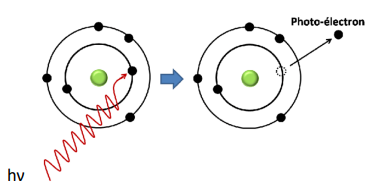
\includegraphics[scale=0.5]{photoelectrique.png}
    \caption{Effet photoélectrique expliqué par les quanta $h\nu$}
\end{figure}
\newline
En 1905, Einstein propose que l'énergie $h\nu$ envoyé à l'atome se convertit en deux énergie différentes: $E_{i}$ l'énergie d'ionisation qui arrache l'électron à la l'atome et $E_{c}$ l'énergie cinétique transmis au photoélectron. On a ainsi : \[ h\nu = E_{i}+E_{c} \geqslant 0 \]
C'est cette énergie $E_{i}$ qui justifie la présence de seuils pour permettre l'effet photoélectrique : si l'énergie $h\nu$ du photon incident (envoyé) est inférieur au seuil $E_{i}$, l'ionisation ne peut pas avoir lieu. Il faut donc augmenter la fréquence, c'est-à-dire diminuer la longueur d'onde du rayonnement électromagnétique.
\newpage
\subsection{Modèle de Bohr}
Le modèle de Bohr ne s'applique qu'aux atomes d'hydrogène et aux hydrogénoïdes (ions de l'atome d'hydrogène), à cause de la présence de plusieurs électrons (l'atome d'hydrogène est le seul atome possèdant un seul électron). Le modèle de Bohr se base sur trois hypothèses faisant appel à des concepts de physique classique:
\begin{enumerate}
    \item Le modèle de l'atome est alors le modèle dit \textit{planétaire}, où l'on considère que les électrons sont présents sur des orbites et gravitent autour du noyau. Bohr postule que l'électron gravite sur des orbites circulaires stables successives (des couches), sans rayonner d'énergie car autrement il s'"effondrerait" sur le noyau.
    \item L'électron ne change d'orbite qu'en absorbant ou en rayonnant une certaine quantité d'énergie.
    \item (Conséquence de (1)) Le moment cinétique de l'électron sur une orbite est constant. Dans ce cours, nous dirons simplement que pour que l'orbite soit stable, elle doit vérifier:
    \[
        mrv = n\frac{h}{2\pi} = n\hbar
        \quad
        \begin{varwidth}{\displaywidth}
            \begin{itemize}[nosep]
                \item m: masse de l'électron (kg)
                \item v: vitesse de l'électron (m$\cdot$s$^{-1}$)
                \item r: le rayon de l'orbite circulaire (m)
                \item h: la constante de Planck (6,62$\times$ 10$^{-34}$ m$^{2}\cdot$kg$\cdot$s$^{-1}$)
                \item n: numéro de la couche électronique (n$\in\mathbb{N^{*}}$)
            \end{itemize}
        \end{varwidth}
    \]
\end{enumerate}
POURQUOI ON UTILISE LE MODELE DE BOHR AVEC PLUSIEURS COUCHES SI ON NE L'UTILISE QUE SUR L'ATOME D'HYDROGENE QUI N'EN POSSEDE QU'UNE ?\newline

On a aussi ces deux relations:
\begin{itemize}
    \item \textbf{Rayons des orbites successives:} $r_{n} = a_{0}n^{2}$ avec $a_{0}$ le rayon de Bohr
    \item \textbf{Énergie de l'électron sur l'orbitale n:} $E_{n} = \frac{E_{1}}{n^{2}}, n\in\mathbb{N^{*}}$; $E_{1}$ l'énergie du niveau fondamental 
\end{itemize}
L'énergie des électrons et le rayon des orbitales successives sont quantifiées.
\begin{figure}[h]
    \centering
    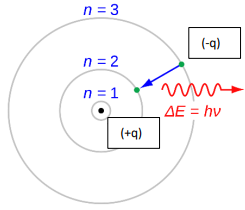
\includegraphics[scale=0.5]{figure_2.png}
    \caption{Quantification des niveaux d'énergie / orbites dans l'atome d'hydrogène}
\end{figure}

On remarque que les énergies des orbitales sont négatives, le niveau d'énergie nulle étant par convention celui où l'atome est ionisé, c'est-à-dire où l'électron n'est plus lié au noyau (n$\rightarrow\infty$).\newpage Ceci implique:
\begin{itemize}
    \item L'énergie d'ionisation $E_{i}$ correspond en fait à la différence entre les énergies de l'état ionisé et de l'état fondamental $E_{i} = E_{final} - E_{initial} = 0 - E_{1} = -E_{1}$
    \item Un électron passe d'une couche n à m en absorbant(excitation)/cédant(désexcitation) de l'énergie (un quanta + précisément). L'échange d'énergie se calcule via la formule suivante :
    \[ \Delta E_{n\to m} = E_{final}-E_{initial} = h\nu = \frac{hc}{\lambda} \]
\end{itemize}

\subsection{Relation de De Broglie}
En 1924, De Broglie propose que chaque particule possède une longueur d'onde associé, se traduisant par la relation suivante \[ \lambda = \frac{h}{p} \] où p est la quantité de mouvement (rappel : p=mv). Cette hypothèse sera appuyé en 1927 lors de la difffraction d'un faisceau d'électrons, mettant en avant la dualité onde-corpuscule des électrons. De Broglie retrouve également les résultats de Bohr sur l'atome d'hydrogène en considérant que les orbites stables sont celles de périmètre multiple de la longueur d'onde de l'électron (L = n$\lambda$), s'affranchissant ainsi du moment cinétique.

\subsection{Principe d'incertitude d'Heisenberg}
L'hypothèse de De Broglie va mener à la notion de "fonction d'onde" d'une particule. De la physique quantique va émerger le \textit{principe d'incertitude d'Heisenberg}:
\[
    \Delta x \Delta p \geqslant \frac{\hbar}{2}
    \quad
    \begin{varwidth}{\displaywidth}
        \begin{itemize}[nosep]
            \item m: masse de l'électron (kg)
            \item v: vitesse de l'électron (m$\cdot$s$^{-1}$)
            \item r: le rayon de l'orbite circulaire (m)
            \item h: la constante de Planck (6,62$\times$ 10$^{-34}$ m$^{2}\cdot$kg$\cdot$s$^{-1}$)
            \item n: numéro de la couche électronique (n$\in\mathbb{N^{*}}$ et n=1 la couche la plus proche du noyau)
        \end{itemize}
    \end{varwidth}
\]
$\Longrightarrow \Delta p = \Delta (mv) = m\Delta v \Longrightarrow m\Delta x\Delta v \geqslant \frac{\hbar}{2}$
\section{Résumé des formules à connaitre}
\subsection{Corps noir}
\subsection{Modèle de Bohr}
\end{document}
